Una señal de sonido no es más que la variación en la presión que ejerce el medio que la transmite sobre su receptor.
La percepción del sonido en los seres humanos ocurre en dos regiones fundamentales: la \textit{periférica} y la \textit{nerviosa}.
Comienza en los oídos y continúa a través de la cóclea, en el oído interno, donde las variaciones en la presión del aire son transformadas en impulsos nerviosos conducidos hacia la corteza cerebral.

El hertz (Hz) es la unidad que expresa la cantidad de vibraciones que emite una fuente sonora en cada segundo de tiempo (frecuencia).
Se considera que el oído humano puede percibir ondas sonoras de frecuencias entre los 20 y los 20~000 Hz.
Los tonos agudos son percibidos en las frecuencias más altas (por encima de 5 kHz), y los graves en las bajas (menos de 250 Hz).

Un sonido puede ser representado de forma simple mediante un \textbf{oscilograma} (figura~\ref{img:oscillogram}), donde el eje X representa el tiempo, y el eje Y representa la \textit{amplitud} de la presión del sonido (generalmente usando unidades de media arbitrarias).
Mediante su análisis se pueden detectar con facilidad los instantes de tiempo de sonido más intensos y aquellos de silencio.

\begin{figure}[!h]
    \centering
    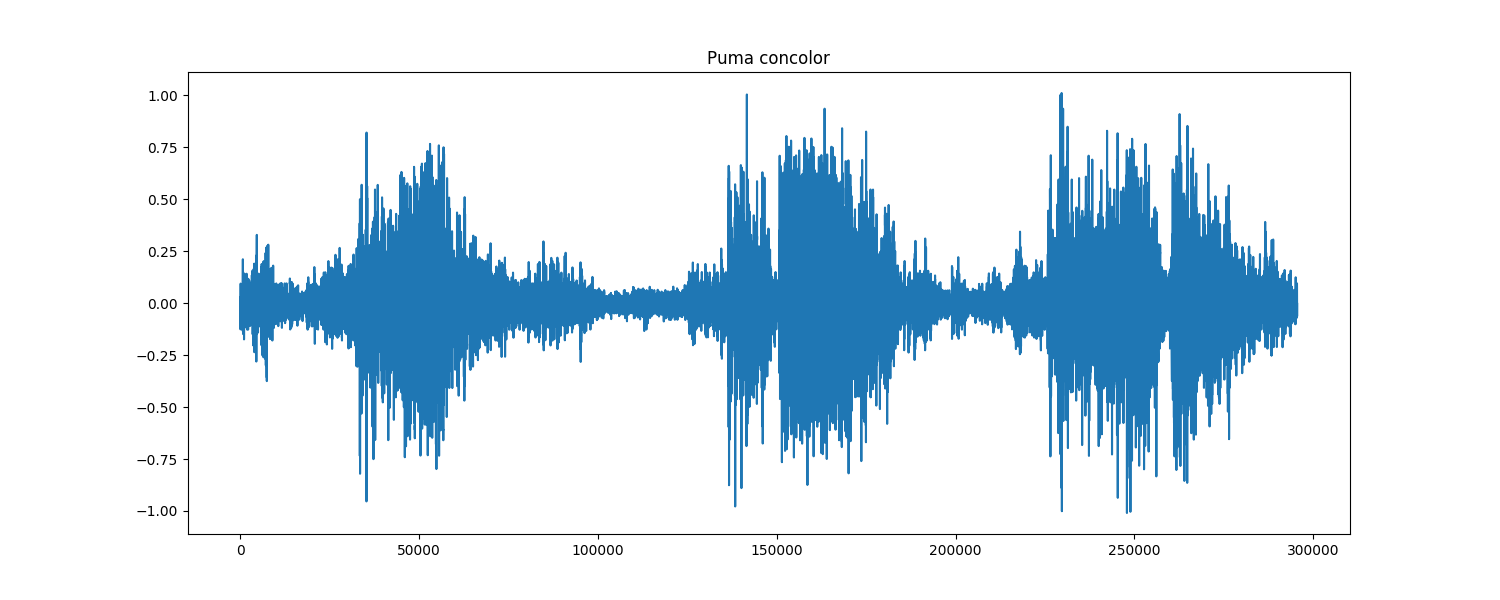
\includegraphics[width=\textwidth]{oscillogram.png}
    \caption{Oscilograma de una vocalización, de 6 segundos de duración, de un individuo de la especie \textit{puma concolor}.}
    \label{img:oscillogram}
\end{figure}

Una importante clase de sonidos son aquellos que consisten en oscilaciones que se repiten periódicamente cada un cierto tiempo.
La duración de una de estas oscilaciones es conocida como su \textit{período} (en segundos) y a la medida inversa se le denomina \textit{frecuencia} (en Hz).
Existen otros sonidos de características aleatorias y que no se repiten periódicamente, llamados \textit{ruidos}.

Una oscilación puede ser descompuesta en una suma de sinusoides elementales de diferentes frecuencias, mediante la aplicación de la \textbf{transformada de Fourier}.
La representación de la transformada de Fourier de una señal en un tiempo dado es conocida como su \textbf{espectro} (figura~\ref{img:spectrum+spectrogram}a).
Esta transformada puede ser igualmente computada sobre pequeñas tramas de tiempo superpuestas, lo que produce una representación tridimensional de la intensidad de las frecuencias en el tiempo, que llamamos \textbf{espectrograma} (figura~\ref{img:spectrum+spectrogram}b).

\begin{figure}[!h]
    \centering
    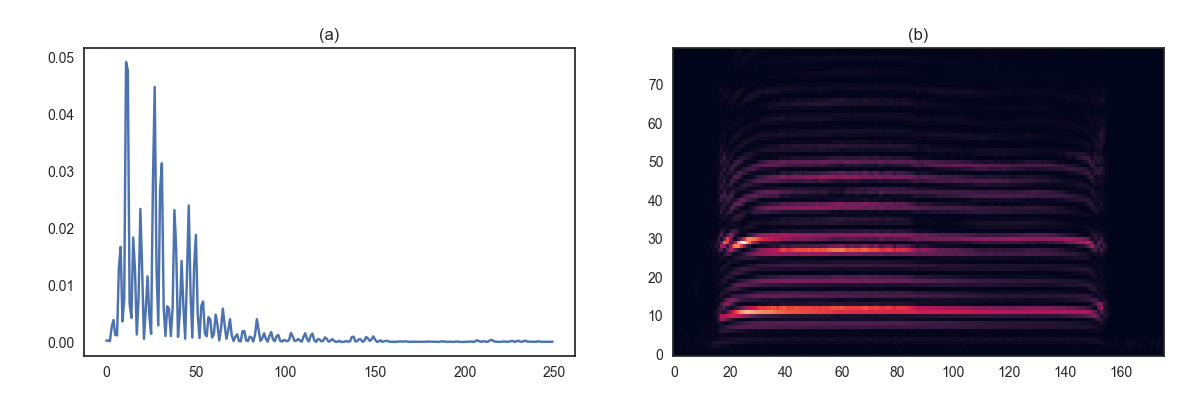
\includegraphics[width=\textwidth]{spectrum+spectrogram.png}
    \caption{Representaciones de la transformada de Fourier de la señal de la figura~\ref{img:oscillogram}: (a) Espectro del segundo 2. (b) Espectrograma.}
    \label{img:spectrum+spectrogram}
\end{figure}

Para el procesamiento computacional de una señal, esta debe ser llevada del dominio analógico al digital, para lo cual se discretiza mediante observaciones realizadas a intervalos regulares.
Los pasos más importantes en esta conversión de la señal de analógica a digital son:

\begin{enumerate}
    \item \textbf{Filtrado}: La señal analógica se filtra con el propósito de limitar las frecuencias presentes al intervalo $[0,B]$, donde $B$ es la frecuencia \textit{máxima} o \textit{de corte}.
    \item \textbf{Muestreo}: Se digitaliza la señal resultante del paso anterior;
    se emplea \textit{frecuencia de muestreo} $F_s = 2B$ para evita el fenómeno de \textit{aliasing}\footnote{Efecto que causa que señales continuas distintas se tornen indistinguibles cuando se muestrean digitalmente si la tasa de muestreo es menor que el doble de la frecuencia más alta.
    Cuando esto sucede, la señal original no puede ser reconstruida de forma unívoca a partir de la señal digital.}.
    \item \textbf{Cuantificación}: La señal digital es cuantificada, se limita el espacio de almacenamiento ocupado por cada muestra.
\end{enumerate}

Para una calidad de audio de CD se emplean valores de muestreo $F_s = 44.1$ kHz y una cuantificación de 16 bits por muestra.

Los algoritmos de inteligencia artificial tradicionalmente operan con vectores numéricos, llamados \textit{vectores de características}.
En las siguientes secciones analizamos los procedimientos mediante los cuales una señal de audio digital se transforma en una secuencia de tales vectores.

Al procesar una grabación sonora, determinados intervalos de tiempo y/o frecuencias pueden resultar más <<importantes>> que otros.
Estas secciones, conocidas como \textit{segmentos}, permiten establecer una correspondencia entre un evento de sonido y un individuo de una especie dada.
La segmentación, por lo tanto, simplifica la tarea de clasificar una señal acústica;
y las operaciones de procesamiento y extracción de características que se mencionan en lo adelante se aplican sobre dichos segmentos.

\section{Tramas}\label{sec:frames}

Para procesar una señal esta a menudo es dividida en pequeños segmentos, conocidos como \textit{tramas}\footnote{\textit{frames} en inglés.}, de longitud constante y espaciados en intervalos de tiempo iguales.
Denotamos por $N$ la cantidad de muestras de la señal que contiene una trama;
de esta forma la duración de una trama será de $N/F_s$.
Asimismo, denotamos por $M$ la cantidad de muestras en que difieren dos tramas consecutivas, conocida como \textit{tamaño de paso}, y que usualmente es menor que $N$.
A partir de estos valores podemos igualmente calcular la cantidad de muestras que dos tramas consecutivas tienen en común, como $N-M$;
y el número de tramas por segundo (\textit{frame rate}) como $F_s/M$.

Cada trama de $N$ muestras es usualmente obtenida mediante la aplicación de una función \textit{ventana} $w(n)$ a la señal, que es distinta de cero solo si $0\leq n\leq N-1$.
Dada la señal $s[n]$, una trama que comienza en la muestra $m$ es obtenida como

\begin{equation}
    \label{eq:windowing}
    s[n]_m = \begin{cases}
                 s[n + m]w(n) & 0\leq n\leq N-1 \\
                 0 & eoc.
    \end{cases}
\end{equation}

Dos de las variantes más conocidas para la función $w(n)$ son las siguientes:

\begin{itemize}
    \item \textbf{Rectangular}:
    \[
        w(n) = \begin{cases}
                   1 & 0\leq n\leq N-1 \\
                   0 & eoc.
        \end{cases}
    \]
    \item \textbf{Hamming}:
    \[
        w(n) = 0.53836 - 0.46164 \cos\left(\frac{2\pi n}{N-1}\right)
    \]
\end{itemize}

La elección de la ventana $w(n)$ tiene un efecto sobre los resultados de operaciones posteriores sobre las tramas obtenidas.
En la práctica, algunos métodos de procesamiento, como la transformada de Fourier producen mejores resultados cuando se emplean funciones que se aproximan a cero en sus extremos, como la de Hamming.

\section{Representaciones Frecuencia-Tiempo}\label{sec:representacionesFrecuencia-tiempo}

El primer paso para el análisis de una señal suele ser su descomposición en frecuencias.
Una trama $x[n]$, de longitud $N$, tiene una representación en dicho dominio que puede ser obtenida mediante la aplicación de la transformada discreta de Fourier (DFT por sus siglas en inglés):

\begin{equation}
    \label{eq:DFT}
    X[f] = \sum_{n=0}^{N-1}{x[n]e^{\frac{-i2\pi fn}{N}}}
\end{equation}

El espectro $X[f]$ puede ser transformado de vuelta al dominio del tiempo aplicando la transformada discreta inversa de Fourier (IDFT):

\begin{equation}
    \label{eq:IDFT}
    x[n] = \frac{1}{N}\sum_{f=0}^{N-1}{X[f]e^{\frac{i2\pi fn}{N}}}
\end{equation}

Al ser $x[n]$ un vector de valores reales, podemos aplicar sobre este una propiedad de la DFT que plantea que el vector $X[f]$ es, por tanto, conjugado simétrico, por lo que suelen considerarse solamente los últimos $\lceil (N+1)/2 \rceil$ valores de este.

Podemos definir $X[f,t]$ como la matriz compuesta por las DFTs correspondientes a cada una de las tramas de una señal, donde el valor en la posición $(f, t)$ corresponde a la amplitud de la frecuencia $f$ en la trama $t$.
A partir de esta matriz se construye el espectrograma de la señal.

\section{Características temporales}\label{sec:característicasTemporales}

Este tipo de características son de las más simples y se computan directamente a partir de la señal digitalizada.
Algunas de las más comunes son:

\begin{enumerate}
    \item \textbf{Short time energy}: Da una medida de la cantidad de energía presente en la señal.
    \[
        STE = \frac{1}{N}\sum_{n=0}^{N-1}{x[n]^2}
    \]
    \item \textbf{Zero crossing rate}: Está dado por el número de veces que la amplitud de la señal cambia de signo.
    \[
        ZCR = \frac{1}{2}\sum_{n=1}^{N-1}{|\text{sign}(x[n]) - \text{sign}(x[n-1])|}
    \]
    donde $\text{sign}(x[n])$ es el signo de la amplitud de la muestra $n$-ésima de la señal.
    \item \textbf{Temporal centroid}: Centro de gravedad del oscilograma.
    \[
        TC = \frac{\sum_{n=0}^{N-1}{n*x[n]}}{\sum_{n=0}^{N-1}{x[n]}}
    \]
    \item \textbf{Temporal width}: Dispersión de las intensidades en torno al centroide.
    \[
        TW = \sqrt{\frac{\sum_{n=0}^{N-1}{(n-TC)^2 x[n]^2}}{\sum_{n=0}^{N-1}{x[n]^2}}}
    \]
    \item \textbf{Temporal flatness}: Da una medida de la variación de la intensidad del sonido en el transcurso del tiempo.
    \[
        TF = \frac{(\prod_{n=0}^{N-1}{|x[n]})^{\frac{1}{N}}}{\frac{1}{N}\sum_{n=0}^{N-1}{x[n]}}
    \]
    Los valores próximos a 1 indican que la intensidad del sonido permanece con poca variación, mientras que lo contrario corresponde a valores cercanos a 0.
    \item \textbf{Autocorrelación}: Coeficientes que pueden ser interpretados como la distribución espectral de la señal en el dominio del tiempo.
    Los primeros $k$ coeficientes pueden ser obtenidos mediante la fórmula
    \[
        R(k) = \frac{\sum_{n=0}^{N-k-1}{x[n]x[n+k]}}{\sqrt{\sum_{n=0}^{N-k-1}{x[n]^2}}\sqrt{\sum_{n=0}^{N-k-1}{x[n+k]^2}}}
    \]
    \item \textbf{Duración}: Longitud del segmento en el tiempo.
    \[
        L = t_{\max} - t_{\min}
    \]
\end{enumerate}

\section{Características espectrales}\label{sec:característicasEspectrales}

Estas características se derivan a partir de la representación de la señal en el dominio de las frecuencias.
Algunas de las más comunes son:

\begin{enumerate}
    \item \textbf{Energía}: Se computa para una frecuencia específica como la suma de los cuadrados de las magnitudes que esta tiene en el tiempo.
    Es, en otras palabras, la suma de los cuadrados del módulo de los valores por cada fila de la matriz $X[f,t]$.
    \item \textbf{Spectral centroid}: Constituye el centroide del espectro de frecuencias.
    \[
        SC = \frac{\sum_{k=0}^{K-1}{f(k)|X[k]|}}{\sum_{k=0}^{K-1}{|X[k]|}}
    \]
    donde $K = \lceil (N+1)/2 \rceil$ es la longitud del vector obtenido aplicando la DFT a la trama, y $f(k)$ frecuencia asociada a la posición $k$-ésima de este.
    \item \textbf{Spectral width}: Medida de la dispersión del espectro de frecuencias en torno a su centroide (SC).
    \[
        SW = \sqrt{\frac{\sum_{k=0}^{K-1}{(f(k)-SC)^2 |X[k]|^2}}{\sum_{k=0}^{K-1}{|X[k]|^2}}}
    \]
    \item \textbf{Spectral flatness}: Permite discriminar si hay eventos harmónicos presentes en la señal o esta se encuentra compuesta solamente por ruido.
    \[
        SF = \frac{(\prod_{k=0}^{K-1}{|X[k]|})^{\frac{1}{K}}}{\frac{1}{K}\sum_{k=0}^{K-1}{|X[k]|}}
    \]
    Los valores de $SF$ próximos a 1 indican que la señal se compone de ruido, mientras que una señal harmónica corresponde a un valor cercano a 0.
    \item \textbf{Spectral roll-off}: Se define como la frecuencia bajo la cual se encuentra un porcentaje específico (usualmente entre el 85\% y el 99\%) de la energía espectral total.
    \item \textbf{Spectral flux}: Caracteriza la variación dinámica de la información espectral.
    Se calcula como la norma de la diferencia entre los espectros de dos tramas consecutivas.
    \item \textbf{Rango de frecuencias}: Máxima ($f_{\max}$) y mínima ($f_{\min}$) frecuencias presentes en la señal.
\end{enumerate}

\section{Mel Frequency Cepstral Coefficients}\label{sec:melFrequencyCepstralCoefficients}

